\section{L6}


\subsection{CPA-secure Encryption}


\paragraph{Pseudorandom Function (PRF)}

Let \(F: \{0, 1\}^n \times \{0, 1\}^n \rightarrow \{0, 1\}^n\) be an efficient length-perserving keyed function. \\
F is a pseudorandom function (PRF) if all PPT distinguisher \(D\), there is a negligible function such that
\[
	| \Pr[D^{F_k(\cdot)}(1^n) = 1] - \Pr[D^{f(\cdot)}(1^n) = 1] | \leq \negl(n)
\]
where \(k \leftarrow \{0,1\}^n\), and \(f \leftarrow \Func_n\) is a random function .

Note that \(\Func_n\) is a set containing all posibilities of \(\{0, 1\}^n \rightarrow \{0, 1\}^n\).

簡而言之,無法區分是否為 random function 的 function,即為 pseudorandom function。

\subparagraph{Quiz}

Show that the size of \(\Func_n\) (aka \(|\Func_n|\)) equals to \(2^{n \cdot 2^n}\).

Ans: \\
The domain \(\{0, 1\}^n\) has \(2^n\) elements, and the codomains \(\{0, 1\}^n\) also has \(2^n\) elements. \\
For each of the \(2^n\) inputs, a function can assign any of \(2^n\) outputs. \\
So the number of such functions is
\[(2^n)^{2^n} = 2^{2 \cdot 2^n}.\]


\paragraph{PRF-based Construction}

這裡的 distinguisher \(D\) 有一個特別的能力,可以詢問 \(F(\cdot)\)(可以將它視為是一種 oracle),而 \(F(\cdot)\) 可能是 PRF \(F_k(\cdot)\) 或是 random function \(f(\cdot)\),但 \(D\) 無法區分到底是哪一種。

\begin{center}
	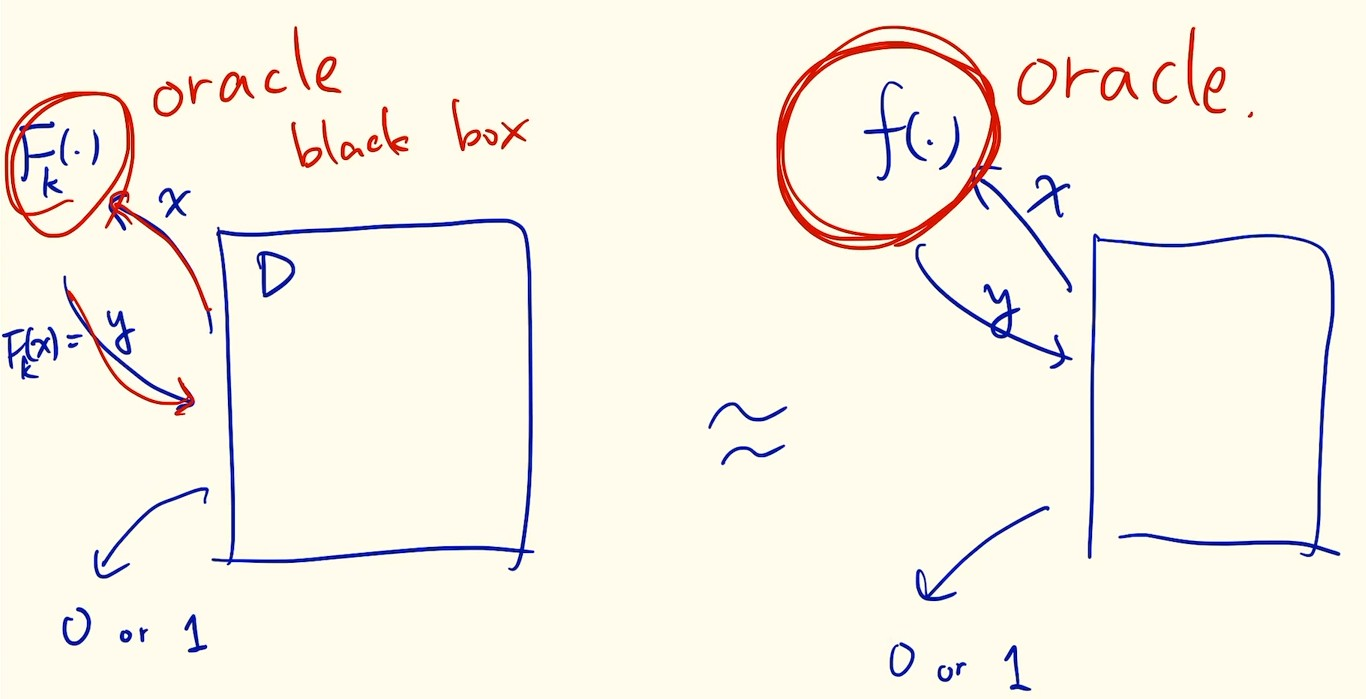
\includegraphics[width=0.8\textwidth, keepaspectratio]{CPA_distinguisher.jpg}
\end{center}

\begin{center}
	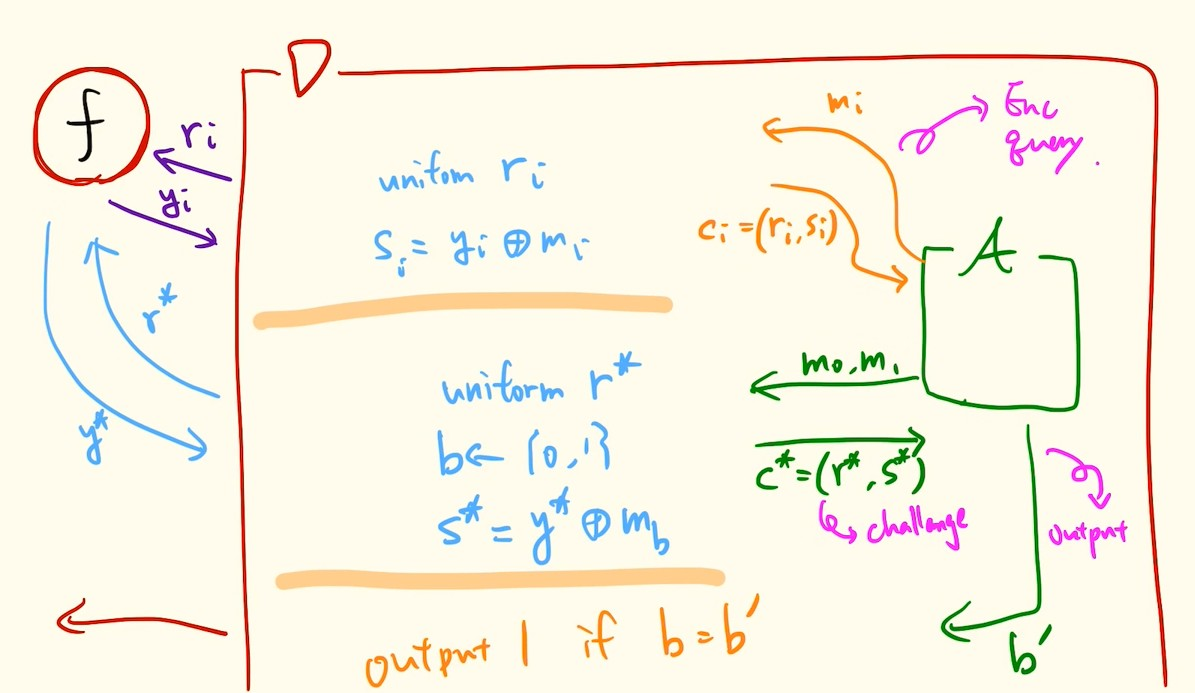
\includegraphics[width=0.9\textwidth, keepaspectratio]{PRF-based_construction.jpg}
\end{center}

Let \(F\) be a PRF and \(\Pi = (\Gen, \Enc, \Dec)\):
\begin{myItemize}
	\item \(\Gen(1^n)\): uniformly choose \(k \in \{0, 1\}^n\) as the key.
	\item \(\Enc(k, m)\): \(m \in \{0, 1\}^n\), uniformly choose \(r \in \{0, 1\}^n\), and compute \(s = F_k(r) \oplus m\) and \(c = (r, s)\).
	\item \(\Dec(k, c)\): parse \(c = (r, s)\), output \(m = F_k(r) \oplus s\)
\end{myItemize}

\begin{theorem}[PRF-based construction is CPA-secure]
	If \(F\) is a PRF, the construction \(\Pi\) is CPA-secure.
\end{theorem}

\subparagraph{證明思路}

Contraposition: If \(\Pi\) is not CPA-secure, then \(F\) is not PRF.

\begin{myProof}
	Let \(\widetilde{\Pi} = (\widetilde{\Gen}, \widetilde{\Enc}, \widetilde{\Dec})\) be one-time pad.

	By modeling \(D\) and \(A\):
	\begin{myEnumerate}[label=(\roman*)]
		\item \[ \Pr[D^{F_k(\cdot)}(1^n) = 1] = \Pr[PrivK^{cpa}_{A, \Pi}(n) = 1]\]
		\item \[ \Pr[D^{f(\cdot)}(1^n) = 1] = \Pr[PrivK^{cpa}_{A, \widetilde{\Pi}}(n) = 1]\]
		\item By assumption,
			\[ | \Pr[D^{F_k(\cdot)}(1^n) = 1] - \Pr[D^{f(\cdot)}(1^n) = 1] | \leq \negl(n) \]
	\end{myEnumerate}
	
	\(\displaystyle \Pr[PrivK^{cpa}_{A, \widetilde{\Pi}}(n) = 1] = ?\)
	\begin{itemize}
		\item Case 1: If \(r^\ast\) is never used in \(\Enc\) query, \(\Pr[A^{case 1}_{win}] = \frac{1}{2}\) \\
		\includegraphics[width=0.7\linewidth, keepaspectratio]{proof_CPA-secure_case1.jpg}
		
		\item Case 2: If \(r^\ast\) is used in \(\Enc\) query, \(\Pr[A^{case 2}_{win}] = 1\) \\
		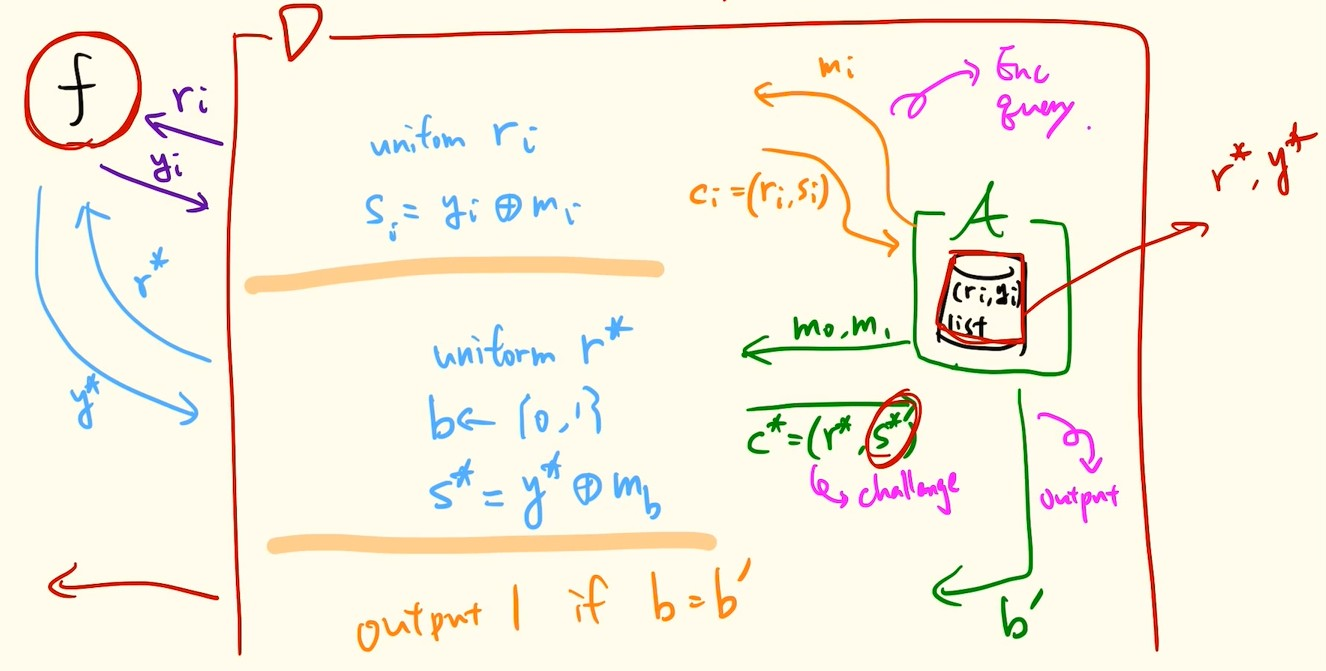
\includegraphics[width=0.7\linewidth, keepaspectratio]{proof_CPA-secure_case2.jpg}
	\end{itemize}
	
	Define an event: \(Repeat\), if \(r^\ast\) is used.
	
	\begin{align*}
		\Pr[PrivK^{cpa}_{A, \compositeaccents{\widetilde}{\Pi}}(n) = 1] &= \Pr[PrivK^{cpa}_{A, \widetilde{\Pi}}(n) = 1 \wedge Repeat] + \Pr[PrivK^{cpa}_{A, \widetilde{\Pi}}(n) = 1 \wedge \neg Repeat] \\
			&\leq \Pr[Repeat] + \Pr[PrivK^{cpa}_{A, \widetilde{\Pi}}(n) = 1 \wedge \neg Repeat] \\
			&= \frac{q(n)}{2^n} + \frac{1}{2} \\
			&= \negl(n) + \frac{1}{2}
	\end{align*}
	
	Use this result to the previous (ii), and then we can get the result of
	\[\Pr[D^{F_k(\cdot)}(1^n) = 1] \leq \frac{1}{2} + \negl(n)\]

\end{myProof}


\subsection{Encryption for Arbitrary Length Message}

CPA-security \(\Rightarrow\) multiple encryption

當我們有任意長度 \(L\) 的訊息需要加密,我們可以對每 \(n\) bit 為一塊的訊息個別進行加密,如此便可以達到加密任意長度訊息的目的。 \\
但前面提到的 CPA-secure 的方法會讓密文長度變成明文長度的兩倍,原本 \(n\)-bit block message 就會變成 \(2n\)-bit ciphertext,最終使得長度為 \(L\) 的訊息在加密後會變成長度的 \(2L\) 的 ciphertext。

接下來會介紹數個解決這問題的方法,統稱為 mode of encryption。


\paragraph{Counter Mode (CTR Mode)}

\(\Enc_k(m_1, \ldots, m_t)\), whose total length is \(n \cdot t\)
\begin{myItemize}
	\item Ramdomly choose \(\mathrm{ctr} \leftarrow \{0, 1\}^n\), set \(c_0 = \mathrm{ctr}\), whose length is \(n\)
	\item For \(i = 1\) to \(t\), compute \(c_i = m_i \oplus F_k(\mathrm{ctr} + i)\), where \(F\) is PRF
	\item Output ciphertext \((c_0, c_1, \ldots, c_t)\), whose length is \(n \cdot (t+1)\)
\end{myItemize}
\begin{center}
	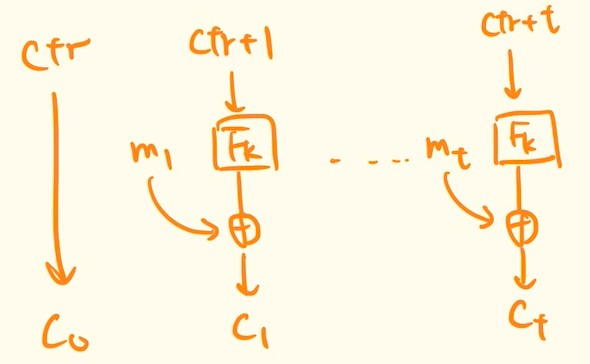
\includegraphics[width=0.3\textwidth, keepaspectratio]{ctr_mode.jpg}
\end{center}

\begin{theorem}
	If \(F\) is PRF, then CTR mode is CPA-secure.
\end{theorem}


\paragraph{Cipher Block Chaining (CBC mode)}

CBC mode is more practical and used in our life.

\(\Enc_k(m_1, \ldots, m_t)\)
\begin{myItemize}
	\item Randomly choose \(c_0 \leftarrow \{0, 1\}^n\)
	\item For \(i = 1\) to \(t\), compute \(c_i = F_k(m \oplus c_{i-1})\)
	\item Output ciphertext \((c_0, c_1, \ldots, c_t)\)
\end{myItemize}

Note that decryption needs \(F_k^{-1}\).

\begin{center}
	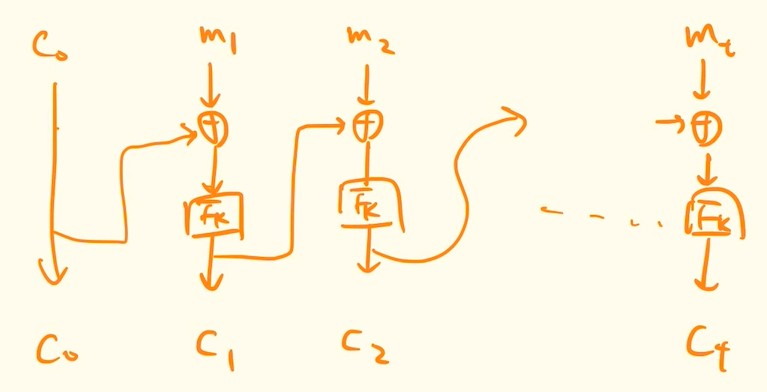
\includegraphics[width=0.5\textwidth, keepaspectratio]{cbc_mode.jpg}
\end{center}

\begin{theorem}
	\(F\) is PRF, CBC mode is CPA-secure.
\end{theorem}

\subparagraph{Quiz}

Show decryptiong of CBC. Draw a flowchart.


\paragraph{Electronic Codebook (ECB mode)}

\(\Enc_k(m_1, \ldots, m_t) \rightarrow F_k(m_1), \ldots, F_k(m_t)\)

Decryption also needs \(F_k^{-1}\).

ECB is not EAV-secure and CPA-secure (\(\because\) ECB is deterministic).

\subparagraph{Quiz}

Prove ECB is not EAV-secure or CPA-secure. \\
寫出 EAV 的攻擊手段。